\chapter{Simulation methods}\label{chap5}

\section{Solutions of Exercises}\label{sec51}
\begin{enumerate}[leftmargin=*]
\item \textbf{Example: The normal model with independent priors}

Let's recap the math test exercise in Chapter \ref{chap4}, this time assuming independent priors. Specifically, let $Y_i \sim N(\mu, \sigma^2)$, where $\mu \sim N(\mu_0, \sigma_0^2)$ and $\sigma^2 \sim IG(\alpha_0 / 2, \delta_0 / 2)$. The sample size is 50, and the mean and standard deviation of the math scores are 102 and 10, respectively. We set $\mu_0 = 100$, $\sigma_0^2 = 100$, and $\alpha_0 = \delta_0 = 0.001$.

\begin{itemize}
	\item Find the posterior distribution of $\mu$ and $\sigma^2$.
	\item Program a Gibbs sampler algorithm and plot the histogram of the posterior draws of $\mu$
\end{itemize}

\textbf{Answer}

The posterior distribution is
\begin{align*}
	\pi(\mu,\sigma^2|\bm{y})&\propto (\sigma^2)^{-N/2}\exp\left\{-\frac{1}{2\sigma^2}\sum_{i=1}^N(y_i-\mu)^2\right\}\\
	&\times \exp\left\{-\frac{1}{2\sigma^2_0}(\mu-\mu_0)^2\right\}\times \left(\frac{1}{\sigma^2}\right)^{\alpha_0/2+1}\exp\left\{-\frac{\delta_0}{2\sigma^2}\right\}.
\end{align*}
Thus, the conditional posterior distribution of $\mu$ is
\begin{align*}
	\pi(\mu,\sigma^2|\bm{y})&\propto \exp\left\{-\frac{1}{2}\left[\frac{1}{\sigma^2}\sum_{i=1}^N(y_i-\mu)^2+\frac{1}{\sigma^2_0}(\mu-\mu_0)^2\right]\right\}\\
	&\propto \exp\left\{-\frac{1}{2}\left[\mu^2\left(\frac{1}{\sigma^2/N}+\frac{1}{\sigma^2_0}\right)-2\mu\left(\frac{\bar{y}}{\sigma^2/N}+\frac{\mu_0}{\sigma_0^2}\right)\right]\right\}.  
\end{align*} 
We set $\mu_n=\sigma^{2}_n\left(\frac{\bar{y}}{\sigma^2/N}+\frac{\mu_0}{\sigma_0^2}\right)$ and $\sigma^{2}_n=\left(\frac{1}{\sigma^2/N}+\frac{1}{\sigma_0^2}\right)^{-1}$. Thus,
\begin{align*}
	\pi(\mu,\sigma^2|\bm{y})&\propto \exp\left\{-\frac{1}{2\sigma_n^2}\left[\mu^2-2\mu\mu_n+\mu_n^2-\mu_n^2\right]\right\}\\
	&\propto \exp\left\{-\frac{1}{2\sigma_n^2}(\mu-\mu_n)^2\right\}.\\  
\end{align*} 
This is the kernel of a normal distribution, that is, $\mu|\sigma^2,\bm{y}\sim N(\mu_n,\sigma_n^2)$.

The conditional posterior distribution of $\sigma^2$ is given by
\begin{align*}
	\pi(\sigma^2|\mu,\bm{y})&\propto (\sigma^2)^{-N/2}\exp\left\{-\frac{1}{2\sigma^2}\sum_{i=1}^N(y_i-\mu)^2\right\}\\
	&\times \left(\frac{1}{\sigma^2}\right)^{\alpha_0/2+1}\exp\left\{-\frac{\delta_0}{2\sigma^2}\right\}\\
	&\propto (\sigma^2)^{-N/2-\alpha_0/2-1} \exp\left\{-\frac{1}{2\sigma^2}\left[\sum_{i=1}^N(y_i-\mu)^2+\delta_0\right]\right\}.
\end{align*} 
Thus, $\sigma^2|\mu,\bm{y}\sim IG(\alpha_n/2,\delta_n/2)$, where $\alpha_n=N+\alpha_0$ and $\delta_n=\sum_{i=1}^N(y_i-\mu)^2+\delta_0=N\hat{\sigma}^2+N(\bar{y}-\mu)^2+\delta_0$ given that $\sum_{i=1}^N(y_i-\bar{y})=0$, where $\bar{y}$ and $\hat{\sigma}$ are the mean and standard deviation estimates.

As we have the conditional posterior distributions, we can use the Gibbs sampling algorithm to perform inference in this model. The following code shows how to do it.

\begin{tcolorbox}[enhanced,width=4.67in,center upper,
	fontupper=\large\bfseries,drop shadow southwest,sharp corners]
	\textit{R code. Gibbs sampler: The math example}
	\begin{VF}
		\begin{lstlisting}[language=R]
rm(list = ls())
set.seed(010101)
N <- 50
# Sample size
muhat <- 102
# Sample mean
sig2hat <- 100
# Sample variance

# Hyperparameters
mu0 <- 100
sig20 <- 100
delta0 <- 0.001
alpha0 <- 0.001

MCMC <- 10000; burnin <- 1000; S <- MCMC + burnin
keep <- (burnin+1):S
# Posterior draws
alphan <- alpha0 + N
sig2Post <- rep(NA, S)
muPost <- rep(NA, S)
sig2 <- sig20
for(s in 1:S){
	sig2n <- (1/(sig2/N)+1/sig20)^(-1)
	mun <- sig2n*(muhat/(sig2/N)+mu0/sig20)
	mu <- rnorm(1, mun, sig2n^0.5)
	muPost[s] <- mu
	deltan <- N*(sig2hat + (muhat - mu)^2)
	sig2 <- invgamma::rinvgamma(1, shape = alphan, rate = deltan)
	sig2Post[s] <- sig2
}
sig2s <- coda::mcmc(sig2Post[keep]) 
mus <- coda::mcmc(muPost[keep]) 
summary(sig2s)
summary(mus)
hist(mus, main = "Histogram: Posterior mean", xlab = "Posterior mean", col = "blue", breaks = 50)
muPost_tq <- quantile(mus, c(0.025, 0.5, 0.975))
muPost_tq
cutoff <- 103
PmuPost_tcutoff <- mean(mus > cutoff)
PmuPost_tcutoff
\end{lstlisting}
	\end{VF}
\end{tcolorbox} 

\begin{figure}[!h]
	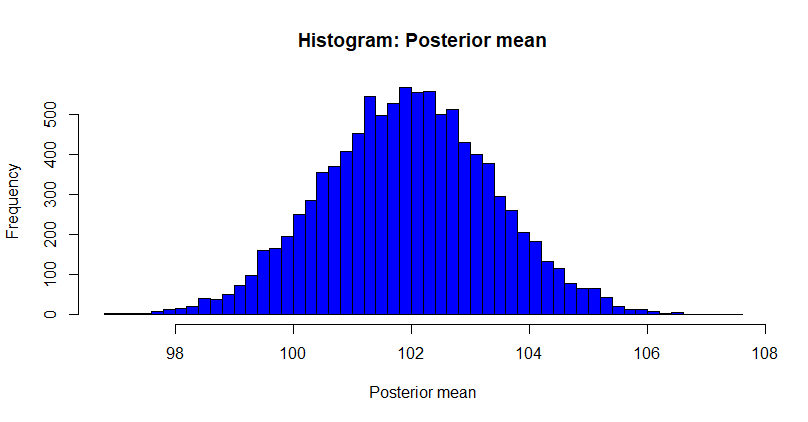
\includegraphics[width=340pt, height=200pt]{Chapters/chapter5/figures/PostMeanMathTest.png}
	%%\centerline{\epsfig{/Chapters/chapter1/figures/cat.eps,width=.8\textheight,height=.4\textwidth}}
	\caption[List of figure caption goes here]{Histogram of posterior draws of mean: Math test}\label{fig51}
\end{figure}

Figure \ref{fig51} shows the histogram of the draws of the posterior mean of the math test results. The posterior mean and median are 101.94 and 101.95, and the 95\% credible interval is (99.14, 104.79).\\

\item Show that the Gibbs sampler is a particular case of the Metropolis-Hastings where the acceptance probability is equal to 1. 

\textbf{Answer}

Without loss of generality let's assume that there are two blocks, $\bm{\theta}=[\bm{\theta}_1 \ \bm{\theta}_2]^{\top}$ such that the Metropolis-Hastings (M-H) algorithm generates a candidate sample $(\bm{\theta}^c_1)$ using a proposal distribution $q(\bm{\theta}^c_1 | \bm{\theta}^{(s-1)})$. The candidate is accepted with probability:
\[
\alpha(\bm{\theta}^{(s-1)}, \bm{\theta}^c) = \min\left\{ 1, \frac{q(\bm{\theta}^{(s-1)}_1 | \bm{\theta}^c) \pi(\bm{\theta}^c | \bm{y})}{q(\bm{\theta}^c_1 | \bm{\theta}^{(s-1)}) \pi(\bm{\theta}^{(s-1)} | \bm{y})} \right\}.
\]

For Gibbs sampling, the candidate $\bm{\theta}^c_1$ is drawn directly from the \emph{full conditional distribution}, so $q(\bm{\theta}^c_1 | \bm{\theta}^{(s-1)}) = \pi(\bm{\theta}^c_1 | \bm{\theta}^{(s-1)}_2, \bm{y})$. Since Gibbs sampling uses the full conditional distributions as the proposal, the key terms simplify. In particular, $q(\bm{\theta}^c_1 | \bm{\theta}^{(s-1)}) = \pi(\bm{\theta}^c_1 | \bm{\theta}^{c}_2, \bm{y})$, and similarly $q(\bm{\theta}^{(s-1)}_1 | \bm{\theta}^c) = \pi(\bm{\theta}^{(s-1)}_1 | \bm{\theta}^{(s-1)}_2, \bm{y})$. Thus, the acceptance probability is given by 
\begin{align*}
	\alpha(\bm{\theta}^{(s-1)}, \bm{\theta}^c) & = \min\left\{ 1, \frac{\pi(\bm{\theta}^{(s-1)}_1 | \bm{\theta}_2^{(s-1)}, \bm{y}) \pi(\bm{\theta}^c | \bm{y})}{\pi(\bm{\theta}^c_1 | \bm{\theta}^{c}_2, \bm{y}) \pi(\bm{\theta}^{(s-1)} | \bm{y})} \right\}\\
	&= \min\left\{ 1, \frac{\pi(\bm{\theta}^{(s-1)}_1 | \bm{\theta}_2^{(s-1)}, \bm{y}) \pi(\bm{\theta}^c_1 | \bm{\theta}^c_2, \bm{y})\pi(\bm{\theta}^c_2 | \bm{y})}{\pi(\bm{\theta}^c_1 | \bm{\theta}^{c}_2, \bm{y}) \pi(\bm{\theta}^{(s-1)}_1 | \bm{\theta}^{(s-1)}_2, \bm{y}) \pi(\bm{\theta}^{(s-1)}_2 | \bm{y})} \right\}\\
	&=1,
\end{align*}
due to $\bm{\theta}^{(s-1)}_2=\bm{\theta}^{c}_2$. Thus, the Gibbs sampling algorithm is implicitly a M-H algorithm where the acceptance probability is 1.

\item Implement a Metropolis-Hastings (M-H) to sample from the Cauchy distribution, $C(0,1)$, using as proposals a standard normal distribution and a Student's t distribution with 5 degrees of freedom. 

\textbf{Answer}

The following code shows to program the M-H to get draws from the Cauchy distribution, $C(0,1)$, using as proposal a standard normal distribution and a Student's t distribution with 5 degree of freedom.

\begin{tcolorbox}[enhanced,width=4.67in,center upper,
	fontupper=\large\bfseries,drop shadow southwest,sharp corners]
	\textit{R code. Metropolis-Hastings algorithm: Cauchy distribution}
	\begin{VF}
		\begin{lstlisting}[language=R]
rm(list = ls()); set.seed(010101)
S <- 100000; df <- 5
theta1 <- runif(S); acept1 <- rep(0, S)
theta2 <- runif(S); acept2 <- rep(0, S)
for (s in 2:S){
	thetac1 <- rnorm(1) # Candidate normal standard
	thetac2 <- rt(1, df = df) # Candidate Students' t
	#Acceptance rate
	a1 <- (dcauchy(thetac1)*dnorm(theta1[s-1]))/(dcauchy(theta1[s-1])*dnorm(thetac1)) 
	a2 <- (dcauchy(thetac2)*dt(theta2[s-1], df = df))/(dcauchy(theta2[s-1])*dt(thetac2, df = df))
	U1 <- runif(1)
	if(U1 <= a1){
		theta1[s] <- thetac1; acept1[s] <- 1
	}else{
		theta1[s] <- theta1[s-1]; acept1[s] <- 0
	}
	if(U1 <= a2){
		theta2[s] <- thetac2; acept2[s] <- 1
	}else{		
		theta2[s] <- theta2[s-1]; acept2[s] <- 0
	}
}
mean(acept1); mean(acept2)
plot(coda::mcmc(theta1)); plot(coda::mcmc(theta2))
h <- hist(theta1, breaks=50, col="blue", xlab="x", main="Cauchy draws from a Metropolis-Hastings algorithm: Normal standard proposal")
pfit <- seq(min(theta1),max(theta1),length=50)
yfit<-dcauchy(pfit)
yfit <- yfit*diff(h$mids[1:2])*length(theta1)
lines(pfit, yfit, col="red", lwd=2)
h <- hist(theta2, breaks=50, col="blue", xlab="x", main="Cauchy draws from a Metropolis-Hastings algorithm: Student's t proposal")
pfit <- seq(min(theta2),max(theta2),length=50)
yfit<-dcauchy(pfit)
yfit <- yfit*diff(h$mids[1:2])*length(theta2)
lines(pfit, yfit, col="red", lwd=2)
\end{lstlisting}
	\end{VF}
\end{tcolorbox} 

Figures \ref{fig52} and \ref{fig53} show the histograms of the posterior draws using the normal and Student's t distributions, along with the density of the Cauchy distribution. The spike in the posterior draws from the standard normal proposal is due to the algorithm being stuck for many iterations at a particular value, as the normal distribution has lighter tails compared to the Cauchy distribution. The convergence using the normal proposal is slower than when using the Student's t proposal, owing to the lighter tails of the former.

\begin{figure}[!h]
	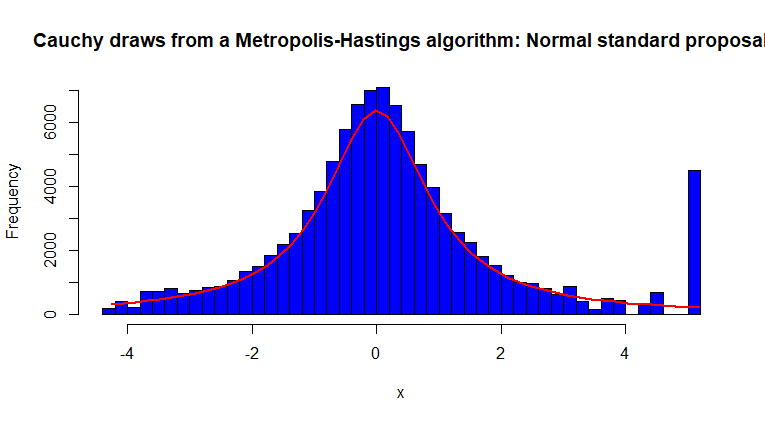
\includegraphics[width=340pt, height=200pt]{Chapters/chapter5/figures/MHnormal.png}
	%%\centerline{\epsfig{/Chapters/chapter1/figures/cat.eps,width=.8\textheight,height=.4\textwidth}}
	\caption[List of figure caption goes here]{Histogram of posterior draws of beta distribution and the density of the beta distribution.}\label{fig52}
\end{figure} 

\begin{figure}[!h]
	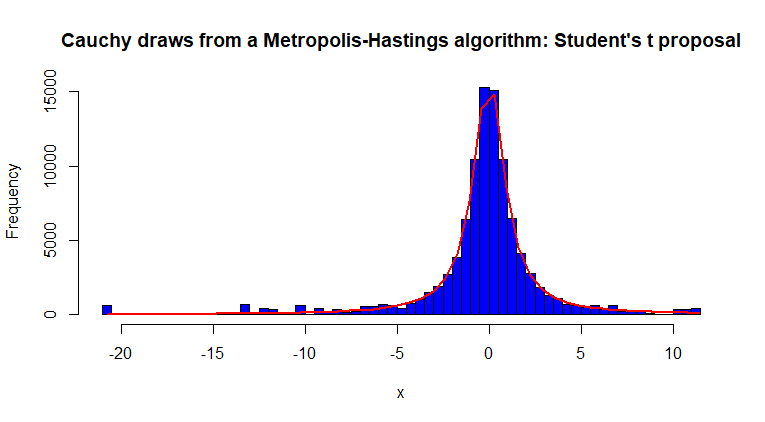
\includegraphics[width=340pt, height=200pt]{Chapters/chapter5/figures/MHt.png}
	%%\centerline{\epsfig{/Chapters/chapter1/figures/cat.eps,width=.8\textheight,height=.4\textwidth}}
	\caption[List of figure caption goes here]{Histogram of posterior draws of beta distribution and the density of the beta distribution.}\label{fig53}
\end{figure} 

\item This exercise was proposed by Professor Hedibert Freitas Lopes, who cites \cite{thomas2021learning} as a useful reference for an introduction to Hamiltonian Monte Carlo in \textbf{R} and the \textit{hmclearn} package. The task is to obtain posterior draws using the Metropolis-Hastings and Hamiltonian Monte Carlo algorithms for the posterior distribution given by 
\[
\pi(\theta_1,\theta_2|\bm{y}) \propto \exp\left\{-\frac{1}{2}(\theta_1^2\theta_2^2 + \theta_1^2 + \theta_2^2 - 8\theta_1 - 8\theta_2)\right\}.
\]
  
  \textbf{Answer}
  
  The following code demonstrates the implementation of the M-H and HMC algorithms for this exercise. For the M-H algorithm, the number of MCMC iterations, burn-in period, and thinning parameters are set to 20,000, 1,000, and 20, respectively. The variance of the proposal distribution is tuned to achieve an acceptance rate close to 25\%. 
  
  For the HMC algorithm, the number of iterations and burn-in period are set to 5,000 and 500, respectively. The step size and number of leapfrog iterations are set to 0.001 and 100, and the mass matrix is defined as \(\bm{M} = \bm{I}_2\). These parameters yield an acceptance rate near 65\%.
  
  Figures \ref{fig54} and \ref{fig55} present the contour plots and posterior draws from the M-H and HMC algorithms for the joint posterior distribution. It can be observed that this distribution is bimodal, and both algorithms successfully capture this feature.
  
 \begin{tcolorbox}[enhanced,width=4.67in,center upper,
 	fontupper=\large\bfseries,drop shadow southwest,sharp corners]
 	\textit{R code. Metropolis-Hastings and Hamiltonian Monte Carlo algorithms}
 	\begin{VF}
 		\begin{lstlisting}[language=R]
rm(list = ls()); set.seed(010101)
# Posterior distribution
PostDist <- function(theta){
	theta1 <- theta[1]; theta2 <- theta[2]
	post <- exp(-0.5*(theta1^2*theta2^2+theta1^2+theta2^2-8*theta1-8*theta2))
	return(post)
}
# Metropolis-Hastings
MH <- function(theta, c2){
	thetac <- MASS::mvrnorm(1, mu = theta, Sigma = c2*diag(2))
	a <- PostDist(thetac)/PostDist(theta)
	U <- runif(1)
	if(U <= a){
		theta <- thetac
		accept <- 1
	}else{
		theta <- theta
		accept <- 0
	}
	return(list(theta = theta, accept = accept))
}
# Posterior draws M-H
S <- 20000; burnin <- 1000; thin <- 20; tot <- S + burnin
K <- 2; c2 <- 1.5
thetaPostMH <- matrix(NA, tot, K)
AcceptMH <- rep(NA, tot)
thetaMH <- c(0, 0)
for(s in 1:tot){
	ResMH <- MH(thetaMH, c2 = c2)
	thetaMH <- ResMH$theta
	thetaPostMH[s,] <- thetaMH
	AcceptMH[s] <- ResMH$accept
}
keep <- seq((burnin), tot, thin)
mean(AcceptMH[keep])
thetaPostMHMCMC <- coda::mcmc(thetaPostMH[keep,])
plot(thetaPostMHMCMC)
coda::autocorr.plot(thetaPostMHMCMC)
# Contour plot
ngrid <- 400
theta1 <- seq(-1, 6, length = ngrid)
theta2 <- seq(-1, 6, length = ngrid)
f <- matrix(0, ngrid, ngrid)
for (i in 1:ngrid){
	for (j in 1:ngrid){
		f[i,j] = PostDist(c(theta1[i],theta2[j]))
	}
}
plot(thetaPostMH[keep,], xlim=range(theta1), ylim=range(theta2), pch=16, col=grey(0.8), xlab=expression(theta[1]), ylab=expression(theta[2]))
contour(theta1,theta2,f, drawlabels=FALSE, add=TRUE, col = "blue", lwd = 1.2)
title("Random walk Metropolis-Hastings")
\end{lstlisting}
 	\end{VF}
 \end{tcolorbox} 

 \begin{tcolorbox}[enhanced,width=4.67in,center upper,
	fontupper=\large\bfseries,drop shadow southwest,sharp corners]
	\textit{R code. Metropolis-Hastings and Hamiltonian Monte Carlo algorithms}
	\begin{VF}
		\begin{lstlisting}[language=R]
HMC <- function(theta, epsilon, L, M){
	Minv <- solve(M); thetat <- theta
	K <- length(thetat)
	mom <- t(mvtnorm::rmvnorm(1, rep(0, K), M))
	logPost_Mom_t <- log(PostDist(thetat)) +  mvtnorm::dmvnorm(t(mom), rep(0, K), M, log = TRUE)  
	theta1 <- theta[1]; theta2 <- theta[2] 
	for(l in 1:L){
		if(l == 1 | l == L){
			mom <- mom + 0.5*epsilon*(-0.5*c(2*theta1*theta2^2+2*theta1-8, 2*theta2*theta1^2+2*theta2-8))
			theta <- theta + epsilon*Minv%*%mom
		}else{
			mom <- mom + epsilon*(-0.5*c(2*theta1*theta2^2+2*theta1-8, 2*theta2*theta1^2+2*theta2-8))
			theta <- theta + epsilon*Minv%*%mom
		}
	}
	logPost_Mom_star <- log(PostDist(theta)) +  mvtnorm::dmvnorm(t(mom), rep(0, K), M, log = TRUE)  
	alpha <- min(1, exp(logPost_Mom_star-logPost_Mom_t))
	u <- runif(1)
	if(u <= alpha){
		thetaNew <- c(theta)
	}else{
		thetaNew <- thetat
	}
	rest <- list(theta = thetaNew, Prob = alpha)
	return(rest)
}
# Posterior draws HMC
S <- 5000; burnin <- 500; tot <- S + burnin
epsilon <- 0.0025;  L <- 100; M <- diag(2)
thetaPostHMC <- matrix(NA, tot, K)
ProbAcceptHMC  <- rep(NA, tot)
thetaHMC <- c(0, 0)
for(s in 1:tot){
	ResHMC <- HMC(theta = thetaHMC, epsilon = epsilon, L = L, M = M)
	thetaHMC <- ResHMC$theta
	thetaPostHMC[s,] <- thetaHMC
	ProbAcceptHMC[s] <- ResHMC$Prob
}
keep <- burnin:S
summary(ProbAcceptHMC[keep])
thetaPostHMCMCMC <- coda::mcmc(thetaPostHMC[keep,])
plot(thetaPostHMCMCMC); coda::autocorr.plot(thetaPostHMCMCMC)
plot(thetaPostHMC[keep,], xlim=range(theta1), ylim=range(theta2), pch=16, col=grey(0.8),
xlab=expression(theta[1]), ylab=expression(theta[2]))
contour(theta1,theta2,f, drawlabels=FALSE, add=TRUE, col = "blue", lwd = 1.2)
title("Hamiltonian Monte Carlo")
\end{lstlisting}
	\end{VF}
\end{tcolorbox} 

 
 \begin{figure}[!h]
 	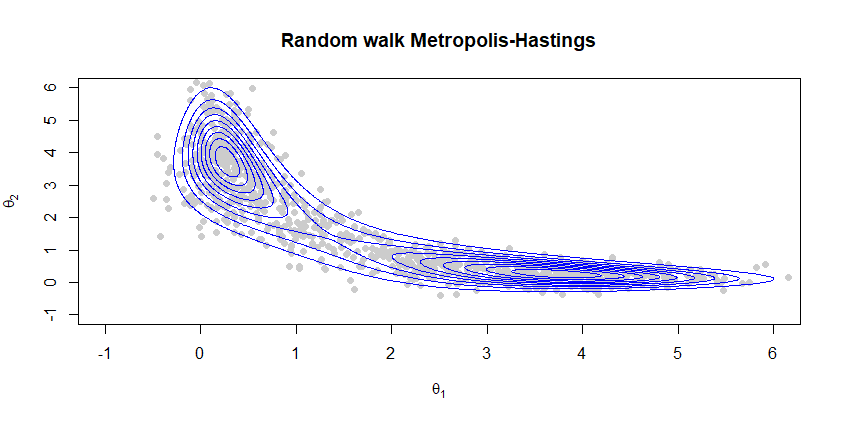
\includegraphics[width=340pt, height=200pt]{Chapters/chapter5/figures/M-Hexample.png}
 	%%\centerline{\epsfig{/Chapters/chapter1/figures/cat.eps,width=.8\textheight,height=.4\textwidth}}
 	\caption[List of figure caption goes here]{Contour plot: Metropolis-Hastings posterior draws.}\label{fig54}
 \end{figure} 
 
 \begin{figure}[!h]
 	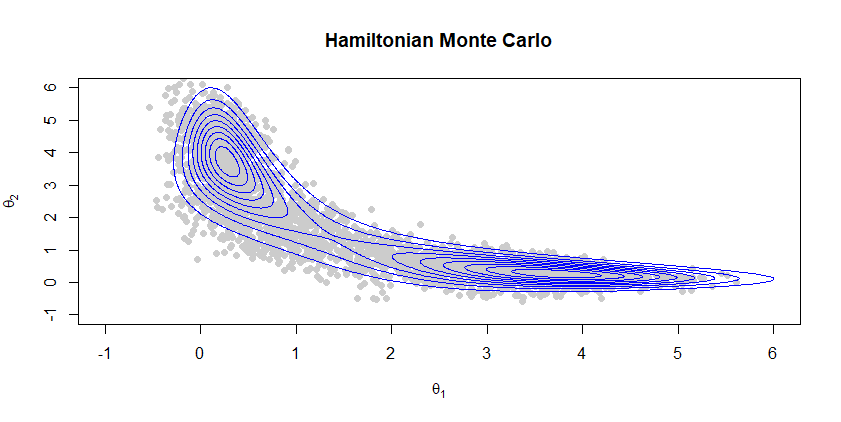
\includegraphics[width=340pt, height=200pt]{Chapters/chapter5/figures/HMCexample1.png}
 	%%\centerline{\epsfig{/Chapters/chapter1/figures/cat.eps,width=.8\textheight,height=.4\textwidth}}
 	\caption[List of figure caption goes here]{Contour plot: Hamiltonian Monte Carlo posterior drwas.}\label{fig55}
 \end{figure} 
 
 \item \textbf{Ph.D. students sleeping hours continues}
 \begin{enumerate}
 	\item Use importance sampling based on a $U(0,1)$ proposal to obtain draws of $\bm{\theta}|\bm{y} \sim B(16.55,39.57)$ in the Ph.D. students' sleeping hours example in Chapter \ref{chap4}. Note that, based on Exercise 15 in Chapter \ref{chap4}, $\alpha_0 = 1.44$ and $\beta_0 = 2.57$.
 	\item Compute the marginal likelihood in this context (Bernoulli-Beta model) and compare it to the result obtained using the Gelfand-Dey method.
 \end{enumerate}

\textbf{Answer}

The posterior distribution of the Bernoulli-beta model is
\begin{align*}
	p(\theta|\bm{y})&=\frac{\prod_{i=1}^N \theta^{y_i}(1-\theta)^{1-y_i}\theta^{\alpha_0-1}(1-\theta)^{\beta_0-1}\Gamma(\alpha_0+\beta_0)}{\Gamma(\alpha_0)\Gamma(\beta_0)p(\bm{y})},
\end{align*}
where 
\begin{align*}
p(\bm{y})&=\int_{\bm{\Theta}}\frac{\prod_{i=1}^N \theta^{y_i}(1-\theta)^{1-y_i}\theta^{\alpha_0-1}(1-\theta)^{\beta_0-1}\Gamma(\alpha_0+\beta_0)}{\Gamma(\alpha_0)\Gamma(\beta_0)}d\theta\\
&=\int_{\bm{\Theta}}\frac{\theta^{\sum _{i=1}^Ny_i+\alpha_0-1}(1-\theta)^{N-\sum_{i=1}^N y_i+\beta_0-1}\Gamma(\alpha_0+\beta_0)}{\Gamma(\alpha_0)\Gamma(\beta_0)}d\theta\\
&=\frac{B(\alpha_n,\beta_n)}{B(\alpha_0,\beta_0)}\int_{\bm{\Theta}}\frac{\theta^{\sum _{i=1}^Ny_i+\alpha_0-1}(1-\theta)^{N-\sum_{i=1}^N y_i+\beta_0-1}}{B(\alpha_n,\beta_n)}d\theta\\
&=\frac{B(\alpha_n,\beta_n)}{B(\alpha_0,\beta_0)}.
\end{align*}
The integral is equal to 1 due to being over the support of $B(\alpha_n,\beta_n)$ distribution.

\begin{tcolorbox}[enhanced,width=4.67in,center upper,
	fontupper=\large\bfseries,drop shadow southwest,sharp corners]
	\textit{R code. Importance sampling: Bernoulli-Beta model}
	\begin{VF}
		\begin{lstlisting}[language=R]
rm(list = ls()); set.seed(010101); S <- 50000
# Importance sampling from standard normal proposal 
an <- 16.55; bn <- 39.57 # Posterior parameters
theta <- runif(S) # Proposal
ws <- dbeta(theta, an, bn) # Weights
wstars <- ws/sum(ws) # Standardized weights
L <- 20000 # Size of posterior sample
thetaBeta <- sample(theta, L, replace = TRUE, prob = wstars) # Posterior draws
# Figure
h <- hist(thetaBeta, breaks=50, col="blue", xlab="x", main="Beta draws from importance sampling: Uniform (0,1) proposal")
pfit <- seq(min(thetaBeta),max(thetaBeta),length=50)
yfit<-dbeta(pfit, an, bn)
yfit <- yfit*diff(h$mids[1:2])*length(thetaBeta)
lines(pfit, yfit, col="red", lwd=2)
a0 <- 1.44; b0 <- 2.57 # Hyperparameters
s <- 15; n <- 52 # Data
LogMarLik <- lbeta(an, bn)-lbeta(a0, b0) # Marginal likelihood
LogMarLik
# Gelfand-Day method
LikPrior <- function(theta){
	Liki <- theta^s*(1-theta)^(n-s)
	Priori <- dbeta(theta, a0, b0)
	LikPriori <- 1 / Liki * Priori 
	return(LikPriori)
}
LogMarLikGD <- log(1/mean(sapply(thetaBeta, LikPrior)))
LogMarLikGD
\end{lstlisting}
	\end{VF}
\end{tcolorbox} 

Figure \ref{fig55} shows the histogram of the posterior draws obtained using the importance sampling algorithm with a uniform proposal. The algorithm performs well. Additionally, the analytic solution for the log marginal likelihood is -32.75, while the Gelfand-Dey method yields -32.76.

\begin{figure}[!h]
	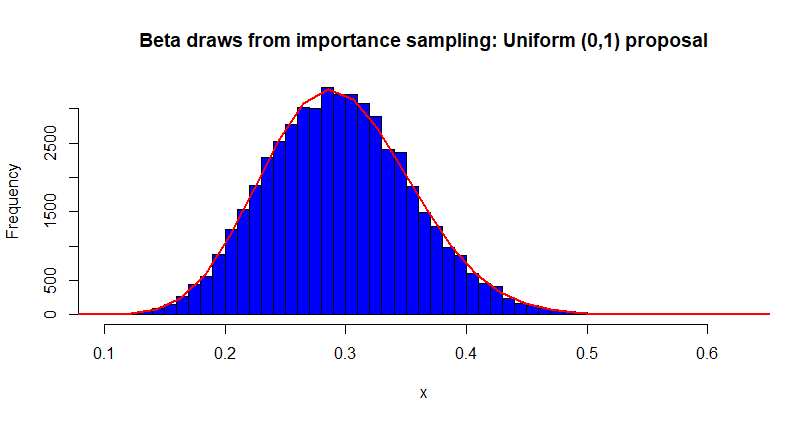
\includegraphics[width=340pt, height=200pt]{Chapters/chapter5/figures/ISbeta.png}
	%%\centerline{\epsfig{/Chapters/chapter1/figures/cat.eps,width=.8\textheight,height=.4\textwidth}}
	\caption[List of figure caption goes here]{Importance sampling: Beta distribution.}\label{fig55}
\end{figure}

\item Example 4.1 in \cite{Gordon1993} is 
\begin{align*}
	\theta_t&=0.5\theta_{t-1}+25\frac{\theta_{t-1}}{1+\theta_{t-1}^2}+8cos(1.2t)+w_t\\
	y_t&=\frac{\theta_{t}^2}{20}+\mu_t,
\end{align*}
where $\theta_0\sim{N}(0,\sqrt{10})$, $w_t\sim\mathcal{N}(0,\sqrt{10})$ and $\mu_t\sim{N}(0,\sqrt{1})$.
\begin{itemize}
	\item Perform sequential importance sampling in this example
	\item Perform particle (Bootstrap) filtering in this example
	\item Estimate the marginal likelihood in this example  
\end{itemize} 

\textbf{Answer}

The following code shows to perform sequential importance sampling and particle (Bootstrap) filtering in the Example 1 in \cite{Gordon1993}. Take into account that we use same strategy as in the dynamic linear model example in the book to calculate the mean and standard deviation of the posterior distribution.

\begin{tcolorbox}[enhanced,width=4.67in,center upper,
	fontupper=\large\bfseries,drop shadow southwest,sharp corners]
	\textit{R code. Sequential importance sampling and particle (Bootstrap) filtering: Gordon (1993) Example 1.}
	\begin{VF}
		\begin{lstlisting}[language=R]
rm(list = ls()); set.seed(010101)
S <- 50000 # Number of particles
sigma_w <- 10^0.5  # State noise
sigma_mu <- 1  # Observation noise
T <- 200 # Sample size
# Simulate true states and observations
theta_true <- numeric(T)
y_obs <- numeric(T)
theta_true[1] <- rnorm(1, mean = 0, sd = sigma_w)  # Initial state
y_obs[1] <- rnorm(1, mean = theta_true[1]^2/20, sd = sigma_mu) 
for (t in 2:T) {
	meant <- 0.5*theta_true[t-1] + 25*(theta_true[t-1]/(1+theta_true[t-1]^2)) + 8*cos(1.2*t)
	theta_true[t] <-  rnorm(1, mean = meant, sd = sigma_w)
	y_obs[t] <- rnorm(1, mean = theta_true[t]^2/20, sd = sigma_mu)  
}
plot(theta_true, type = "l"); plot(y_obs, type = "l")
# Sequential Importance Sampling (SIS)
particles <- matrix(0, nrow = S, ncol = T) 
weights <- matrix(0, nrow = S, ncol = T) 
weightsSt <- matrix(0, nrow = S, ncol = T) 
# Initialization
particles[, 1] <- rnorm(S, mean = 0, sd = sigma_w)
weights[, 1] <- dnorm(y_obs[1], mean = particles[, 1]^2/20, sd = sigma_mu)
weightsSt[, 1] <- weights[, 1] / sum(weights[, 1])
# Sequential updating
for (t in 2:T) {
	particles[, t] <- rnorm(S, mean = 0.5*particles[, t-1] + 25*(particles[, t-1]/(1+particles[, t-1]^2)) + 8*cos(1.2*t), sd = sigma_w)  # Compute weights
	weights[, t] <- weightsSt[, t-1] * dnorm(y_obs[t], mean = particles[, t]^2/20, sd = sigma_mu)
	weightsSt[, t] <- weights[, t] / sum(weights[, t])
}
FilterDist <- colSums(particles * weightsSt)
SDFilterDist <- (colSums(particles^2 * weightsSt) - FilterDist^2)^0.5
library(dplyr); library(ggplot2); library(latex2exp)
ggplot2::theme_set(theme_bw())
df <- tibble(t = 1:T, mean = FilterDist, lower = FilterDist - 2*SDFilterDist, upper = FilterDist + 2*SDFilterDist, theta_true = theta_true)
plot_filtering_estimates <- function(df) {
	p <- ggplot(data = df, aes(x = t)) + geom_ribbon(aes(ymin = lower, ymax = upper), alpha = 1, fill = "lightblue") + geom_line(aes(y = theta_true), colour = "black", alpha = 1, linewidth = 0.5) + geom_line(aes(y = mean), colour = "blue", linewidth = 0.5) + ylab(TeX("$\\theta_{t}$")) + xlab("Time")
	print(p)
}
plot_filtering_estimates(df)
\end{lstlisting}
	\end{VF}
\end{tcolorbox} 

\begin{tcolorbox}[enhanced,width=4.67in,center upper,
	fontupper=\large\bfseries,drop shadow southwest,sharp corners]
	\textit{R code. Sequential importance sampling and particle (Bootstrap) filtering: Gordon (1993) Example 1.}
	\begin{VF}
		\begin{lstlisting}[language=R]
# Particle filtering
particles <- matrix(0, nrow = S, ncol = T) 
particlesT <- matrix(0, nrow = S, ncol = T)
weights <- matrix(0, nrow = S, ncol = T) 
weightsSt <- matrix(0, nrow = S, ncol = T) 
weightsSTT <- matrix(1/S, nrow = S, ncol = T) 
logalphas <- matrix(0, nrow = S, ncol = T) 
# Initialization
particles[, 1] <- rnorm(S, mean = 0, sd = sigma_w)  # Sample initial particles
weights[, 1] <- dnorm(y_obs[1], mean = particles[, 1]^2/20, sd = sigma_mu)  # Importance weights
weightsSt[, 1] <- weights[, 1] / sum(weights[, 1])  # Normalize weights
ind <- sample(1:S, size = S, replace = TRUE, prob = weightsSt[, 1]) # Resample 
particles[, 1] <- particles[ind, 1] # Resampled particles
particlesT[, 1] <- particles[, 1] # Resampled particles
# Sequential updating
pb <- winProgressBar(title = "progress bar", min = 0, max = T, width = 300)
for (t in 2:T) {
	# Propagate particles
	particles[, t] <- rnorm(S, mean = 0.5*particles[, t-1] + 25*(particles[, t-1]/(1+particles[, t-1]^2)) + 8*cos(1.2*t), sd = sigma_w)
	# Compute weights
	logalphas[, t] <- dnorm(y_obs[t], mean = particles[, t]^2/20, sd = sigma_mu, log = TRUE) 
	weights[, t] <- exp(logalphas[, t])
	weightsSt[, t] <- weights[, t] / sum(weights[, t])
	if(t < T){
		ind <- sample(1:S, size = S, replace = TRUE, prob = weightsSt[, t])
		particles[, 1:t] <- particles[ind, 1:t]
	}else{
		ind <- sample(1:S, size = S, replace = TRUE, prob = weightsSt[, t])
		particlesT[, 1:t] <- particles[ind, 1:t]
	}
	setWinProgressBar(pb, t, title=paste( round(t/T*100, 0), "% done"))
}
close(pb)
FilterDist <- colSums(particles * weightsSt)
SDFilterDist <- (colSums(particles^2 * weightsSt) - FilterDist^2)^0.5
FilterDistT <- colSums(particlesT * weightsSTT)
SDFilterDistT <- (colSums(particlesT^2 * weightsSTT) - FilterDistT^2)^0.5
\end{lstlisting}
	\end{VF}
\end{tcolorbox}  

\begin{tcolorbox}[enhanced,width=4.67in,center upper,
	fontupper=\large\bfseries,drop shadow southwest,sharp corners]
	\textit{R code. Sequential importance sampling and particle (Bootstrap) filtering: Gordon (1993) Example 1.}
	\begin{VF}
		\begin{lstlisting}[language=R]
library(dplyr); library(ggplot2); library(latex2exp)
ggplot2::theme_set(theme_bw())
df <- tibble(t = 1:T, mean = FilterDist, lower = FilterDist - 2*SDFilterDist, upper = FilterDist+ 2*SDFilterDist, meanT = FilterDistT, lowerT = FilterDistT - 2*SDFilterDistT,
upperT = FilterDistT + 2*SDFilterDistT, x_true = theta_true)
plot_filtering_estimates <- function(df) {
	p <- ggplot(data = df, aes(x = t)) + geom_ribbon(aes(ymin = lower, ymax = upper), alpha = 1, fill = "lightblue") + geom_line(aes(y = x_true), colour = "black", alpha = 1, linewidth = 0.5) + geom_line(aes(y = mean), colour = "blue", linewidth = 0.5) +
	geom_line(aes(y = meanT), colour = "purple", linewidth = 0.5) + ylab(TeX("$\\theta_{t}$")) + xlab("Time")
	print(p)
}
plot_filtering_estimates(df)
MargLik <- colMeans(weights)
plot(MargLik, type = "l", xlab = "Time", ylab = "Marginal likelihood", main = "Marginal likelihood")
\end{lstlisting}
	\end{VF}
\end{tcolorbox} 
Figure \ref{fig56} shows the true trajectory of the state vector (black line), the posterior mean (blue line), and the $\pm2\hat{\sigma}_{\theta}$ posterior estimate (light blue shaded area) from the sequential importance sampling algorithm. We observe that there is no light blue shaded area after time period 40, and the algorithm exhibits poor performance after $t=75$. This is due to weight degeneracy.

Figure \ref{fig57} shows the performance of particle filtering (see Figure 3 in \cite{Gordon1993}). There is the true state vector (black line), the means based on $\left\{\bm{\theta}_{1:t}^{(s)},w_t^{*(s)}\right\}$ (blue line) and  $\left\{\bm{\theta}_{1:t}^{r(s)},1/S\right\}$ (purple line), and the area defined by $\pm2\hat{\sigma}_{\theta}$ based on the former (light blue shaded area). Note that the particle filtering algorithm has better performance than the SIS algorithm. This is due to restarting the system every stage by resampling, which in turn mitigates the weight degeneracy issue.

Finally, Figure \ref{fig58} shows the posterior estimate of marginal likelihood based on the particle filtering algorithm.

\begin{figure}[!h]
	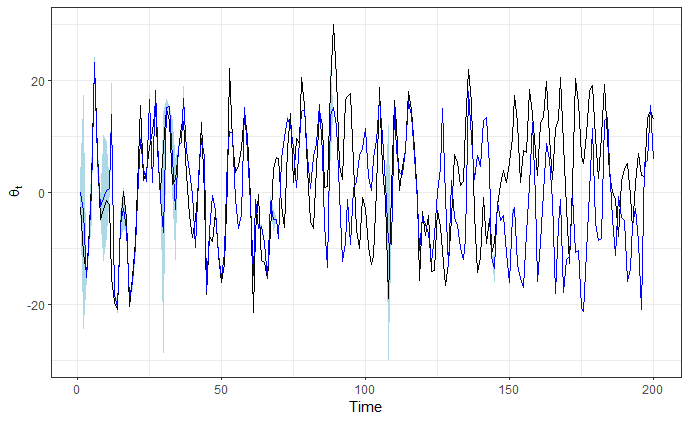
\includegraphics[width=340pt, height=200pt]{Chapters/chapter5/figures/SISGordon.png}
	%%\centerline{\epsfig{/Chapters/chapter1/figures/cat.eps,width=.8\textheight,height=.4\textwidth}}
	\caption[List of figure caption goes here]{Sequential importance sampling: Example 1, \cite{Gordon1993}.}\label{fig56}
\end{figure} 

\begin{figure}[!h]
	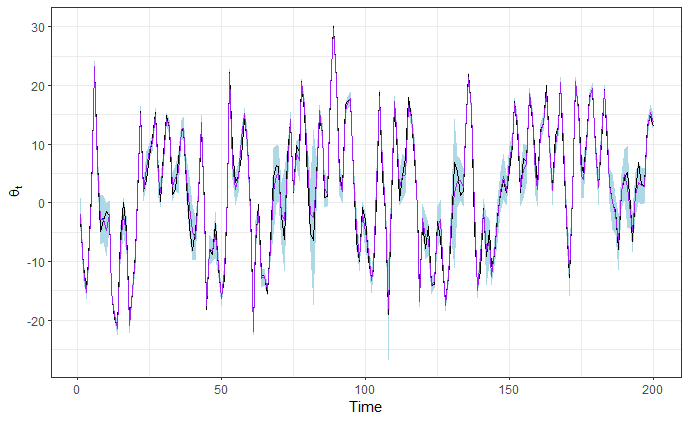
\includegraphics[width=340pt, height=200pt]{Chapters/chapter5/figures/PFGordon.png}
	%%\centerline{\epsfig{/Chapters/chapter1/figures/cat.eps,width=.8\textheight,height=.4\textwidth}}
	\caption[List of figure caption goes here]{Particle (Bootstrap) filtering: Example 1, \cite{Gordon1993}.}\label{fig57}
\end{figure}

\begin{figure}[!h]
	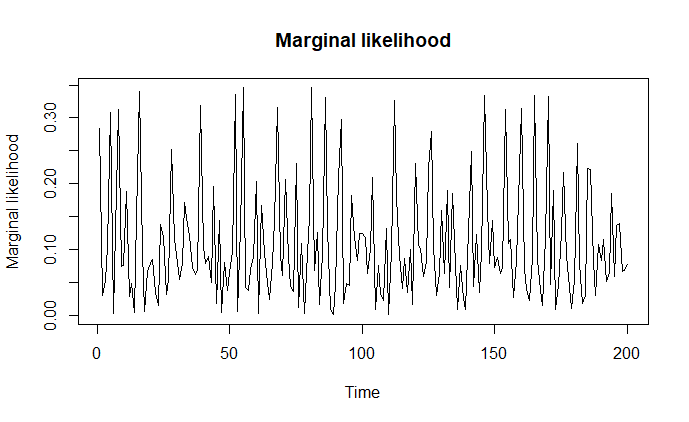
\includegraphics[width=340pt, height=200pt]{Chapters/chapter5/figures/MarLikGordon.png}
	%%\centerline{\epsfig{/Chapters/chapter1/figures/cat.eps,width=.8\textheight,height=.4\textwidth}}
	\caption[List of figure caption goes here]{Marginal likelihood: Example 1, \cite{Gordon1993}.}\label{fig58}
\end{figure}

\item \textbf{Ph.D. students sleeping hours continues}

\begin{itemize}
	\item Perform the diagnostics of Section 4.4 in this example.
	\item Check if there are errors in the posterior simulator of the Metropolis-Hastings algorithm in this example using the Geweke approach using as test functions the first moments of $p$ and $p^2$. Remember from Exercise 15 in Chapter \ref{chap4} that the sample size is 52, and $\alpha_0=1.22$ and $\beta_0=2.57$.
	\item Run the Geweke test using $\alpha_0=2.57$ and $\beta_0=1.22$, and check the results.
\end{itemize}

\textbf{Answer}

We initially run the Metropolis-Hastings (M-H) algorithm for 100,000 iterations and obtain an effective sample size of 13,606. The naive and time-series standard errors are 0.00019 and 0.00052, respectively, indicating correlation—a feature also observed in the autocorrelation plot (not shown). However, the trace plot appears satisfactory. The Geweke test statistic is 1.97, marginally rejecting the null hypothesis that the means of the first 10\% and the last 50\% of the posterior draws are equal. Additionally, the dependence factor is 6.1, which exceeds the rule-of-thumb threshold of 5. The posterior draws pass both stages of Heidelberger and Welch's convergence diagnostic.

Given the autocorrelation issues, we set a burn-in period of 20,000 iterations and apply a thinning parameter of 10. Figures \ref{fig59} and \ref{fig510} display the trace and autocorrelation plots of the posterior draws. We observe that the draws appear stationary around their mean, and the autocorrelation decreases rapidly to zero.

The naive and time-series standard errors are 0.00068 and 0.00072, respectively. The similarity between these values indicates a low level of autocorrelation, consistent with the results in Figure \ref{fig510}. The effective sample size of the posterior draws is 7,066, while the total number of posterior draws is 8,000.

The Geweke test statistic is 0.23, providing no statistical evidence to reject the null hypothesis of equal means in the two segments of the posterior draws. The Raftery and Lewis test yields a dependence factor close to 1, indicating minimal dependence. The Heidelberger and Welch test does not reject the null hypothesis of stationarity for the posterior draws and confirms that the mean is both accurate and stable.

Then, we implement the proposal by \cite{geweke2004getting} to assess the reliability of the posterior simulator. We use as test functions the first moments of $p$ and $p^2$. We fail to reject the null hypothesis of equal means across the two test functions, indicating that the posterior simulator is functioning correctly. To evaluate the effectiveness of the test, we run the \textit{marginal-conditional simulator} with prior parameters $\alpha_{0} = 1.22$ and $\beta_{0} = 2.57$. In contrast, for the \textit{successive-conditional simulator}, we use prior parameters $\alpha_{0} = 2.57$ and $\beta_{0} = 1.22$. In this case, we reject the null hypothesis in the two test functions, suggesting that the test performs well in this example.

\begin{tcolorbox}[enhanced,width=4.67in,center upper,
	fontupper=\large\bfseries,drop shadow southwest,sharp corners]
	\textit{R code. Metropolis-Hastings algorithm: Ph.D. students sleeping hours.}
	\begin{VF}
		\begin{lstlisting}[language=R]
rm(list = ls()); set.seed(010101); an <- 16.55; bn <- 39.57
S <- 100000; p <- runif(S); accept <- rep(0, S)
for (s in 2:S){
	pc <- runif(1)
	a <- dbeta(pc, an, bn)/dbeta(p[s-1], an, bn)
	U <- runif(1)
	if(U <= a){	p[s] <- pc; accept[s] <- 1
	}else{p[s] <- p[s-1]; accept[s] <- 0}
}
library(coda); library(latex2exp)
thetaPost <- mcmc(p)
plot(thetaPost, density = FALSE, main = "Trace plot", ylab = "Proportion")
autocorr.plot(thetaPost, main = "Autocorrelation plot")
summary(thetaPost); effectiveSize(thetaPost) 
geweke.diag(thetaPost, frac1 = 0.1, frac2 = 0.5)
raftery.diag(thetaPost, q = 0.025, r = 0.005, s = 0.95)
heidel.diag(thetaPost, eps = 0.1, pvalue = 0.05)
burnin <- 20000; thin <- 10; keep <- seq(burnin, S, thin)
thetaPostNew <- mcmc(p[keep])
plot(thetaPostNew, density = FALSE, main = "Trace plot", ylab = "Proportion")
autocorr.plot(thetaPostNew, main = "Autocorrelation plot")
summary(thetaPostNew); effectiveSize(thetaPostNew) 
geweke.diag(thetaPostNew, frac1 = 0.1, frac2 = 0.5)
raftery.diag(thetaPostNew, q = 0.025, r = 0.005, s = 0.95)
heidel.diag(thetaPostNew, eps = 0.1, pvalue = 0.05)
# Marginal-conditional simulator
a0 <- 1.22; b0 <- 2.57; ThetaPrior <- rbeta(S,a0,b0) 
yPrior <- rbinom(S, 1, prob = ThetaPrior)
parsmcmc1 <- coda::mcmc(cbind(ThetaPrior, ThetaPrior^2))
Summ1 <- summary(parsmcmc1)
# Successive-conditional simulator
N <- 52
SucConSim <- function(a0, b0, par){
	y <- rbinom(N, 1, prob = par)
	an <- a0 + sum(y); bn <- b0 + N - sum(y); pc <- runif(1)
	a <- dbeta(pc, an, bn)/dbeta(par, an, bn); U <- runif(1)
	if(U <= a){par <- pc}else{par <- par}
	return(par)
}
a0 <- 1.22; b0 <- 2.57 # a0 <- 2.57; b0 <- 1.22
par2 <- rbeta(1, a0, b0); pars2 <- rep(NA, S); pars2[1] <- par2
for(s in 2:S){
	Res <- SucConSim(a0 = a0, b0 = b0, par = pars2[s-1])
	pars2[s] <- Res
}
parsmcmc2 <- coda::mcmc(cbind(pars2, pars2^2))
Summ2 <- summary(parsmcmc2)
TestGeweke <- function(j){
	Test <- (Summ1[["statistics"]][j,1] - Summ2[["statistics"]][j,1])/(Summ1[["statistics"]][j,4]+Summ2[["statistics"]][j,4])^0.5
	Reject <- abs(Test) > qnorm(0.975); return(list(Test = Test, Reject = Reject))
}
TestGeweke(1); TestGeweke(2)
\end{lstlisting}
	\end{VF}
\end{tcolorbox} 

\begin{figure}[!h]
	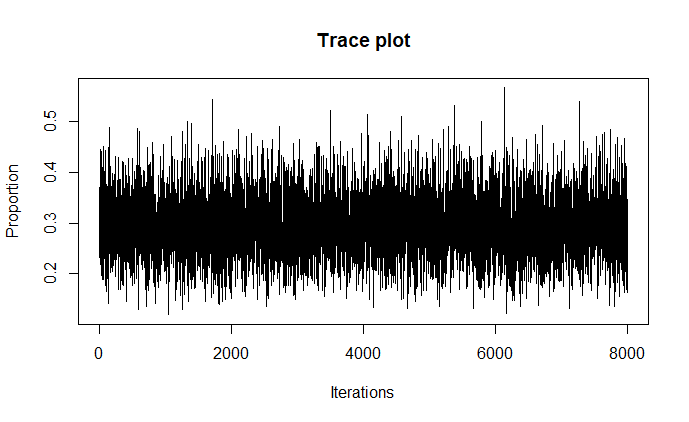
\includegraphics[width=340pt, height=200pt]{Chapters/chapter5/figures/TracePlotProp}
	\caption[List of figure caption goes here]{Trace plot of posterior draws: Proportion of students that sleep at least 6 hours.}\label{fig59}
\end{figure}

\begin{figure}[!h]
	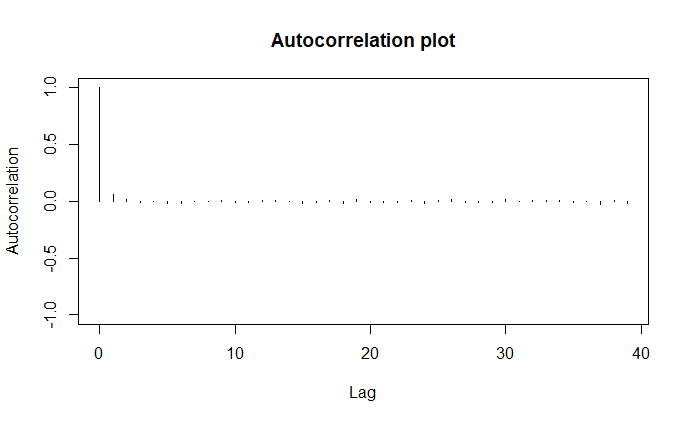
\includegraphics[width=340pt, height=200pt]{Chapters/chapter5/figures/AutocorrPlotProp.png}
	\caption[List of figure caption goes here]{Autocorrelation plot of posterior draws: Proportion of students that sleep at least 6 hours.}\label{fig510}
\end{figure}
  

\end{enumerate}